\documentclass[twocolumn, a4paper]{./ieicejsp_tokai}
%%%%%%%%%%%%%%%%%%%%%%%%%%%%%%%%%%%%%%%%%%%%%%%%%%%%%%%%%%%%%%%%%%%%%%%%%%%%
%2012.02.28:ページ当りの図表の数を増加した.
%------------------------------------

%------------------------------------
%   Common   Added Sekine 
%------------------------------------
\newcommand{\Eqn}[1]{&\hspace{-0.6em}#1\hspace{-0.6em}&}
%------------------------------------
%07.07.03--parameterを追加
\newcommand{\figoneb}[8]{ %
\begin{figure}[#1]\vspace{#4}
\begin{center}
\includegraphics[width=#2\linewidth,height=#3\linewidth]{#5}
\end{center}
\vspace{#6}
%%\caption{{\large #7}}
\caption{{#7}}
\label{#5}
\vspace{#8}
\end{figure}}
%------------------------------------
\newcommand{\figminipage}[6]{ %
\begin{minipage}{#1\linewidth}\begin{center}
\includegraphics[width=#2\linewidth,height=#3\linewidth]{#4}\\[#5]
{{\small #6}}
\end{center}
\vskip0pt
\end{minipage}
}
%-------------------------------------------------
\newcommand{\bmath}[1]{\mbox{\boldmath $#1$}}
\newcommand{\bm}[1]{\mbox{\boldmath ${#1}$}}      %07.11.06
\newcommand{\brm}[1]{\mbox{\boldmath ${\rm#1}$}}      %07.11.06
\newcommand{\diag}[1]{\mbox{\/ \rm diag$\left(#1 \right)$}}
\newcommand{\MAT}[4]{\left(\begin{array}{cc}
       \displaystyle{#1}  & \displaystyle{#2} \\
      \displaystyle{#3}  & \displaystyle{#4} 
\end{array}\right)}
\newcommand{\VEC}[2]{\left(\begin{array}{c}
       \displaystyle{#1}  \\
       \displaystyle{#2} 
\end{array}\right)}
\newcommand{\VECT}[2]{\left(\begin{array}{cc}
       \displaystyle{#1} \displaystyle{#2} 
\end{array}\right)}
\newcommand{\noseplist}[1][2.5]{\usecounter{enumii} \topsep=0pt \parsep=0pt \itemindent=0zw \leftmargin=#1zw \labelwidth=#1zw \labelsep=0.5zw \itemsep=0pt}
\newcommand{\sm}[1]{\mbox{\small ${#1}$}}
\newcommand{\fts}[1]{\mbox{\footnotesize ${#1}$}}

%-------------------------------------------------
%96.08.21--図表の入れ方を変更(美文書作成13.5.8 p198参照)
\setcounter{topnumber}{6}    %ページ上部の図表は2個まで(2->3)
\def\topfraction{.98}        %ページの上7割まで図表で占めて可(.7->.98)
\setcounter{bottomnumber}{6} %ページ下部の図表は1個まで(1->3)
\def\bottomfraction{.98}     %ページの下3割まで図表で占めて可(.3->.98)
\setcounter{totalnumber}{10}  %ページ当たりの図表は3個まで(3->4)
\def\textfraction{.02}       %ページの2割は本文にする(.2->.02)
\def\floatpagefraction{.98}  %図表だけのページは少なくとも5割を
                               % 図表が占める(0.5->0.98)
\setcounter{dbltopnumber}{5}
\def\dbltopfraction{.98}
\def\dblfloatpagefraction{.98}
%-------------------------------------------------

%\usepackage[dvips]{graphicx}
\usepackage[dvipdfmx]{graphicx}
\usepackage{bm,subfigure,amsmath,float}
\usepackage{subfig}
\usepackage{multirow,array}
\usepackage{tabularx}
\newcolumntype{C}{>{\centering\arraybackslash}X}
\newcolumntype{L}{>{\raggedleft\arraybackslash}X}
\newcolumntype{R}{>{\raggedright\arraybackslash}X}
\usepackage{comment}
\usepackage{amsmath}
\usepackage{amsfonts}
%%\usepackage[dviout]{graphicx}
\usepackage{color}
\usepackage{amsmath}
%\usepackage{amssymb}
%\usepackage{amsxtra}

\title{{コンプレッシブバイラテラルフィルタの任意レンジカーネル拡張}
}
  \author{
    %角谷 勇仁 (指導教員:福嶋 慶繁) \\ 名古屋工業大学 工学部
  }

\begin{document}
\maketitle

\section{まえがき}
カーネルの半径に依存しない定数時間バイラテラルフィルタ (O(1) BF)のひとつであるコンプレッシブバイラテラルフィルタ (CBF)~\cite{compressiveBF}は処理が軽量で性能が高いがレンジカーネルにガウス関数しか使用できないという制約がある.本論文では,任意のレンジカーネルに拡張する方法を提案し,その性能を評価する.
%
\section{O(1) BF}
通常のBFの処理は以下の式で定義される.
\begin{align}
\bar{I}(\bm{p}) =\frac{\sum_{\bm{q}\in N(\bm{p})}w_{s}(\bm{p},\bm{q})w_{r}(\bm{I}(\bm{p}),\bm{I}(\bm{q}))\bm{I}(\bm{q})}{\sum_{\bm{q}\in N(\bm{p})}w_{s}(\bm{p},\bm{q})w_{r}(\bm{I}(\bm{p}),\bm{I}(\bm{q}))}
\label{eq:bailateral}
\end{align}
ここで,$\hat{I_p}, I_p, I_q$はそれぞれ出力画素, 注目画素,参照画素を表しており,$w_{s}(p,q)=e^{\frac{-(q-p)^{2}}{2\sigma_{s}^{2}}}$, $w_{r}(I_p,I_q)=e^{\frac{-(I_q-I_p)^{2}}{2\sigma_{r}^{2}}}$である.
定数時間バイラテラルフィルタは,$w_{r}(\bm{a},\bm{b})\approx\sum{_{k=0}^{K-1}}\phi_{k}(\bm{a})\psi_{k}(\bm{b})$と変数分離しこれを式~\eqref{eq:bailateral}に代入し,式変形することでカーネル半径に依存しない定数時間での処理が可能となる.
%
\section{CBF}
CBFでは,フーリエ級数展開によりレンジカーネルを近似し,三角関数の加法定理を用いて以下のように変数分離する.
\begin{align}
  w_r(a,b) \approx \alpha_{0} + 2\sum_{k=1}^{K}\alpha_{k}(\cos(w_{k}a)\cos(w_{k}b) \nonumber\\
  +\sin(w_{k}a)\sin(w_{k}b))
  \label{eq:cosdecomposition}
\end{align}
ここで,ガウシアンカーネルのフーリエ級数は$\alpha_{k} \approx \frac{2}{T}e^{-\frac{1}{2}(\frac{2\pi}{T}k\sigma_{r})^{2}}$である.これを式~\eqref{eq:bailateral}に代入して整理することにより,4K+1回の畳み込み回数での処理が可能となる.
さらに,式\eqref{eq:bailateral}と$I_{p}$の差分をとると
\begin{align}
 \hat{I}_{\bm{p}}\!-\!I_{\bm{p}} = \frac{\sum_{\bm{q}\in\mathcal{S}} w_s(\bm{p},\bm{q})w_r(I_{\bm{p}},I_{\bm{q}})(I_{\bm{q}} - I_{\bm{p}})
}{\sum_{\bm{q}\in\mathcal{S}} w_s(\bm{p},\bm{q})w_r(I_{\bm{p}},I_{\bm{q}})}
\label{eq:bilateral-subform}
\end{align}
と表される.レンジカーネルはガウス関数であるので,その微分を利用すると$\sigma_{r}^{2}w'_{r}(a,b) = w_{r}(a,b)(b-a)$という式を満たし,これを式~\eqref{eq:bilateral-subform}に代入し変数分離することで畳み込み回数を2K回まで削減できる.
%
\section{提案手法}
$w_r(a,b)(b-a)$は偶関数と奇関数の積であることから,奇関数であることを利用するとフーリエ正弦級数展開と三角関数の加法定理を利用することで以下のように変数分離できる.
\begin{align}
  w_{r}(a,b)(b-a) \approx 2\sum_{k=1}^{K}b_{k}(\sin(\omega_{k}a)\cos(\omega_{k}b) \nonumber  \\
    -\cos(\omega_{k}a)\sin(\omega_{k}b)). \label{eq:compressive-sin-decomp}
\end{align}

これと式~\eqref{eq:cosdecomposition}を式\eqref{eq:bilateral-subform}に代入することで畳み込み回数2K回で,任意のレンジカーネルを利用することが可能となる.周期Tは,レンジカーネルとその近似値の二乗誤差が最小になるように決定する.提案手法では,二乗誤差を求める際,0 $\sim I_{range}$までの誤差を一次元ループで求め,周期Tと誤差の分布の関係から黄金分割探索法で最小値を決定することで高速な処理時間を実現する.
%
\section{実験}
本実験では,提案手法 (proposed method),特異値分解による手法 (SVD)~\cite{SVD}, 線形補間による手法 (Linear)~\cite{linear}の三つの手法を比較する.図~\ref{processing_time},\ref{PSNR}は各手法の畳み込み回数に応じた処理時間,8枚の画像に対するPeak Signal-to-Noise Ratio (PSNR)の平均値を示している.なおレンジカーネルに$f(x)=e^{\frac{-x^{6}}{6\sigma_{r}^{6}}}$を用いたときの結果である.提案手法は,Linearと同程度の処理時間で,SVDとほぼ同じ性能を実現できた.
%
\begin{figure}[H]
 \begin{center}
  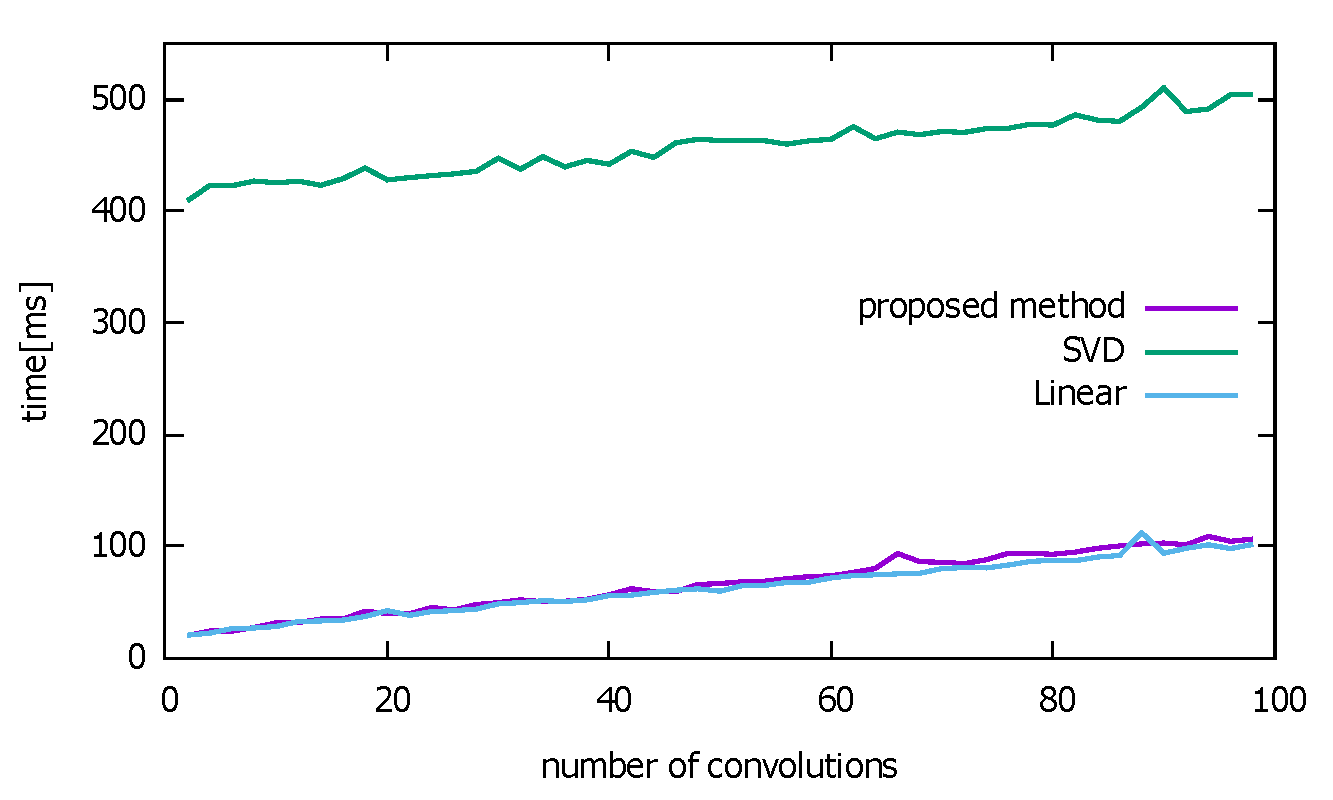
\includegraphics[scale = 0.22]{fig/processing_time.pdf}
  \caption{各手法の処理時間}
  \label{processing_time}
 \end{center}
\end{figure}

\begin{figure}[H]
 \begin{center}
  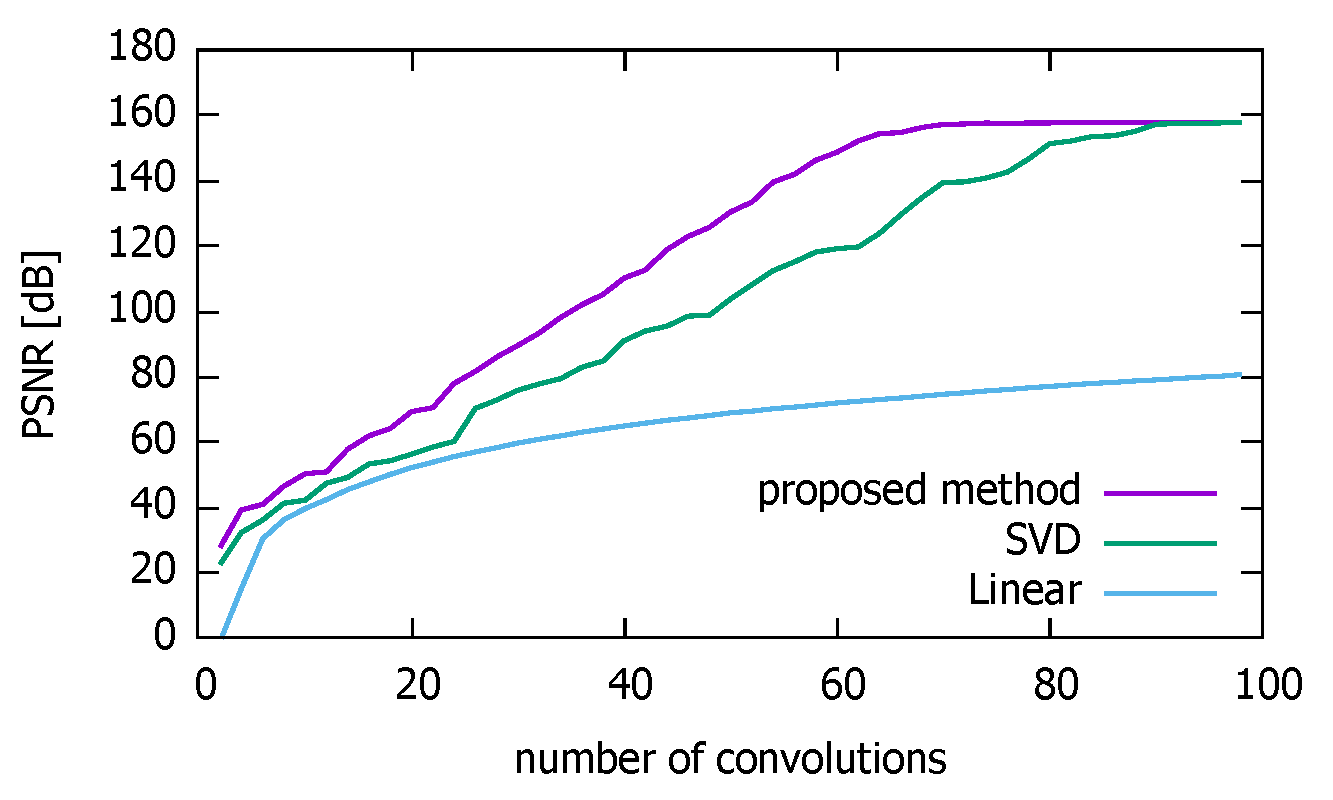
\includegraphics[scale = 0.22]{fig/6-gauss_PSNR.pdf}
  \caption{各手法のPSNR ($\sigma_r=40, \sigma_s=5$)}
  \label{PSNR}
 \end{center}
\end{figure}
%
\section{むすび}
提案手法により,CBFを任意のレンジカーネルに拡張し,Linearとほぼ同じ処理時間でSVD以上の性能を実現できた.
{\small
\begin{thebibliography}{9}
\baselineskip=9.5pt
\bibitem{compressiveBF}
K. Sugimoto and S. Kamata, ``Compressive bilateral filtering,'' in \emph{IEEE Transactions on Image Processing}, 2015.

\bibitem{SVD}
K. Sugimoto and N. Fukushima and S. Kamata ``200 FPS Constant-Time Bilateral Filter Using SVD and Tiling Strategy,,'' in \emph{in Proc. IEEE International on Image Processing (ICIP)}, 2019.

\bibitem{linear}
Q. Yang and K.H. Tan and N. Ahuja, ``Real-time o(1) bilateral filtering, '' in \emph{IEEE Conference on Computer Vision and Pattern Recognition (CVRP)}, 2017.
\end{thebibliography}
}
\end{document}
